\chapter{Artificial Absorption\ }
\label{chap:artificial_absorption}
Variance reduction is a mechanism by which the probabilities and
weights of the Monte Carlo problem are modified to improve the
performance of a given estimator. In the context of improving MCSA
results, such modifications may potentially introduce bias into the
system. However, using Monte Carlo within an MCSA iterative scheme
provides a potential buffer for the solution from this bias as the
correction generated by the Monte Carlo solve will contain large
statistical error even without variance reduction.

The random walk sequences generated by the adjoint Neumann Ulam
decomposition in Eqs~(\ref{eq:adjoint_probability}) and
(\ref{eq:adjoint_weight}) will continue on indefinitely without the
implementation of a weight cutoff procedure (which in itself is
effectively a form of biased variance reduction). This is due to the
fact that all states to which a stochastic history may move in a given
transition exist within the system and have a non-zero weight. A
simple variance reduction scheme is to introduce \textit{artificial
  absorption} into the system such that at each transition event, a
stochastic history will now have some finite probability of being
terminated through absorption as well as transitioning to other states
in the system. This probability, $p_{abs}$, modifies the probabilities
and weights in the adjoint random walk sequence as:
\begin{equation}
  p_{ij} = \frac{|h_{ji}|}{\sum_j|h_{ji}|}(1-p_{abs})\:,
  \label{eq:absorption_probabilities}
\end{equation}
and
\begin{equation}
  w_{ij} = \frac{sign(h_{ji})}{(1-p_{abs})}\sum_j|h_{ji}|\:.
  \label{eq:absorption_weights}
\end{equation}
At each transition step, a history at state $i$ will then sample the
probability distribution function generated by
Eq~(\ref{eq:absorption_probabilities}) with an additional absorption
state added to the distribution. If the sampling procedure results in
a transition to the absorption state, the history is immediately
terminated. The advantages of this for residual Monte Carlo are that
increasing the absorption probability decreases the length of each
random walk (resulting in speedup), while the random walk has a higher
weight contribution at every step. This higher weight means that each
history is depositing more information near its birth site which will
on average be located where the system residual is the largest. An
additional advantage of this formulation is that the full Neumann-Ulam
decomposition is maintained.

To observe the effects of this variance reduction on MCSA solutions,
the transient Poisson problem was again solved with the adjoint
method, this time with varying values of artificial absorption. A $200
\times 200$ grid was used with 40,000 histories at every iteration
with the expected value estimator converged to a tolerance of
\sn{1}{-8}. To reduce the effect of the weight cutoff on this study,
the weight cutoff was set to \sn{1}{-12} such that it is significantly
more likely that a history will be terminated by absorption rather
than weight cutoff. Figure~\ref{fig:absorption_iters} gives the number
of iterations to converge as a function of the artificial absorption
probability. Up to a probability of roughly 0.5, the iterative
performance is not significantly affected with the information lost
due to shortened random walks causing a small increase in the number
of iterations. At a probability of 0.6, the number of iterations
required grows rapidly as the shortened randow walks create an MCSA
correction that has a larger statistical error. Convergence was
observed to be lost at probabilities of 0.7 and higher.

The random walk length has a strong effect on CPU time as
well. Figure~\ref{fig:absorption_time} gives the CPU time in seconds
required to converge as a function of artificial absorption
probability. Initially, small absorption probabilities not only
maintain iterative performance, but also drastically reduced the time
required to converge as absorption was more frequent than even a large
weight cutoff but the weights themselves were not significantly
modified. As the number of iterations grow rapidly, so does the time
required to converge to a solution. Based on these results, using a
small amount of artificial absorption should provide some CPU speedup
while maintaining iterative performance.

\begin{figure}[t!]
  \centering
  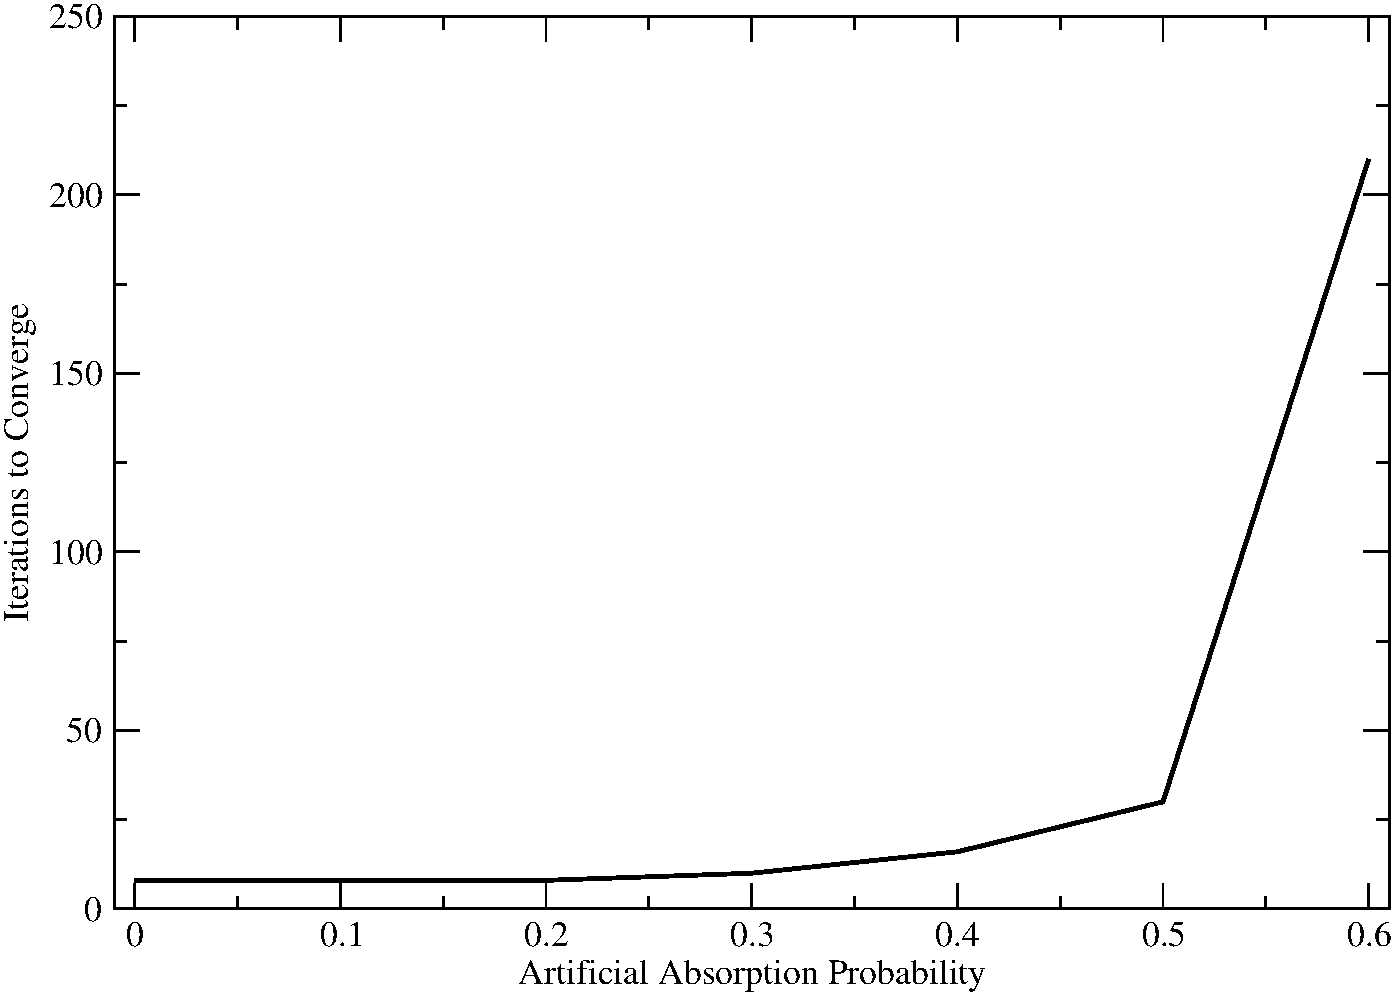
\includegraphics[width=4.5in,clip]{chapters/mc_background/absorption_iters.pdf}
  \caption{\textbf{Iterations (s) to converge vs. artificial
      absorption probability for a $200 \times 200$ square mesh and
      40,000 histories.}  \textit{The addition of absorption is
      detrimental to iterative performance due to both the shortening
      of the random walks as well as the modification of the
      transition weight.}}
  \label{fig:absorption_iters}
\end{figure}

\begin{figure}[t!]
  \centering
  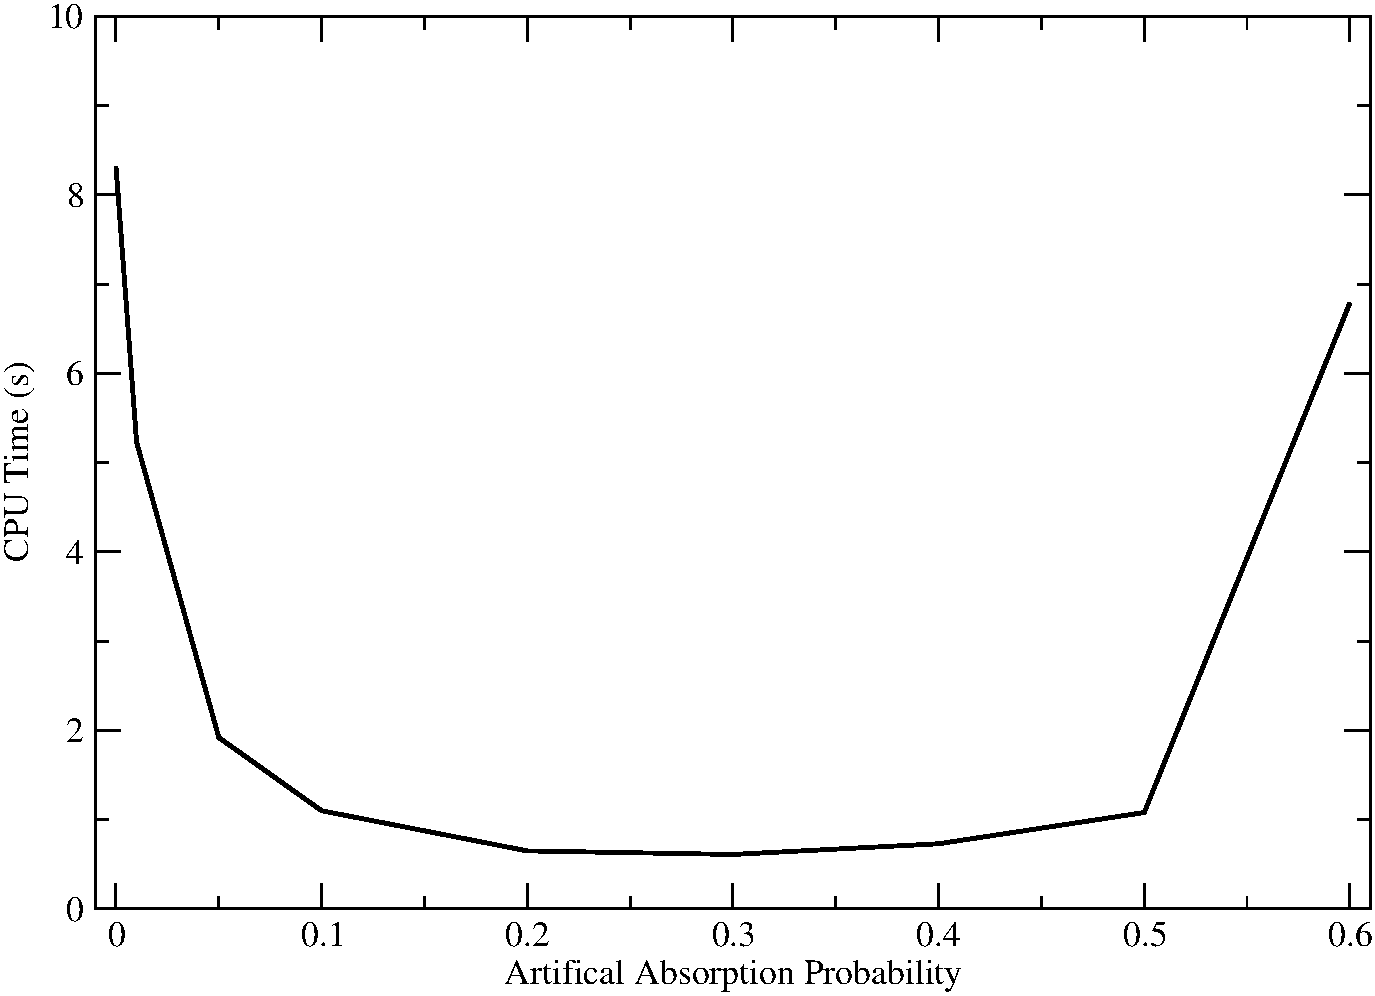
\includegraphics[width=4.5in,clip]{chapters/mc_background/absorption_time.pdf}
  \caption{\textbf{CPU Time (s) to converge vs. artificial absorption
      probability for a $200 \times 200$ square mesh and 40,000
      histories.}  \textit{The reduced random walk length speeds up
      the calculation with a fixed number of histories. Too much
      artificial absorption increases iterations rapidly giving an
      increasing CPU time.}}
  \label{fig:absorption_time}
\end{figure}
